%!TEX program = xelatex
\documentclass{beamer}

\usepackage{blindtext}

\usetheme{Execushares}

\title{Structured Sparsity in\\Numerical Optimisation}
\subtitle{Universit\'{e} C\^ote D'Azur, Inria, France}
\author{Matteo Frigo}
\date{Nice - December 4, 2017}

\setcounter{showSlideNumbers}{1}

\usepackage{amsmath,amssymb,amsfonts,amsthm}

\newcommand{\HH}{\mathcal{H}}
\newcommand{\NN}{\mathbb{N}}
\newcommand{\ZZ}{\mathbb{Z}}
\newcommand{\QQ}{\mathbb{Q}}
\newcommand{\RR}{\mathbb{R}}
\newcommand{\rd}{\mathbb{R}^d}
\newcommand{\CC}{\mathbb{C}}
\newcommand{\norm}[1]{\left\|#1\right\|}
\newcommand{\normtwosq}[1]{\left\|#1\right\|_2^2}
\newcommand{\onehalf}{\frac{1}{2}}
\newcommand {\matlab} {$\text{Matlab}^{\circledR}$\,}
\newcommand {\expect} {\mathbb{E}}
\newcommand {\prob} {\mathbb{P}}
\renewcommand{\epsilon}{\varepsilon}
%\renewcommand{\theta}{\vartheta}
%\renewcommand{\rho}{\varrho}
\renewcommand{\phi}{\varphi}
\hyphenation{sub-dif-fe-ren-tial}
\hyphenation{COMMIT}

\DeclareMathOperator*{\argmin}{argmin}


\begin{document}
	\setcounter{showProgressBar}{0}
	\setcounter{showSlideNumbers}{0}

	\frame{\titlepage}

	\begin{frame}
		\frametitle{Contents}
		\begin{enumerate}
			\item Mathematics \\ \textcolor{ExecusharesGrey}{\footnotesize\hspace{1em} Proximal Operator, FISTA, Regularisation}
			\item Model Design  \\ \textcolor{ExecusharesGrey}{\footnotesize\hspace{1em} Sparsity, Hierarchy, Lasso}
			\item Brain Imaging \\ \textcolor{ExecusharesGrey}{\footnotesize\hspace{1em} Tractography, dMRI, Connectomics}
		\end{enumerate}
	\end{frame}

	\setcounter{framenumber}{0}
	\setcounter{showProgressBar}{1}
	\setcounter{showSlideNumbers}{1}
	\section{Mathematics}
	
		\begin{frame}
			\frametitle{Numerical Optimisation}
			\begin{itemize}
			\item $\HH$ is a set
			\item $\Phi: \HH\to\RR$
			\item Find \begin{equation}\nonumber x^* = \argmin_{x\in\HH}\Phi(x)\end{equation}
			\end{itemize}
			
			\pause
			\vfill
			
			Our setting:
			\begin{itemize}
			\item $\HH=\rd$
			\item $\Phi(x) := f(x) + g(x)$
				\begin{itemize}
				\item $f(x)$ is convex and has $L$-Lipschitz continuous gradient
				\item $g(x)$ is convex and lower semi-continuous
				\end{itemize}
			\item Find \begin{equation}\nonumber x\in\rd = \argmin_{x\in\rd}f(x)+g(x)\end{equation}
			\end{itemize}
			
		\end{frame}

		\begin{frame}
			\frametitle{Trivial case}
			\begin{minipage}{.45\textwidth}
			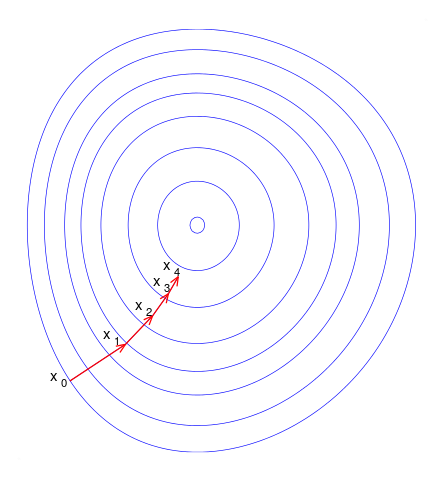
\includegraphics[width=\textwidth]{img/gradientdescent}
			\end{minipage}\qquad
			\begin{minipage}{.45\textwidth}
			Smooth case: $g(x) = 0$
			\begin{equation}\nonumber
			x^*=\argmin_{x\in\rd}f(x).
			\end{equation}
			Scheme:
			\begin{equation}
			\nonumber
			x^+ = x - \gamma\nabla f(x)
			\end{equation}
			where $\gamma=\frac{1}{L}$
			\end{minipage}
		\end{frame}

		\begin{frame}
		\frametitle{Constrained optimisation}
		Let $C\subset\rd$,
		\begin{equation}
		\nonumber
		x^*=\argmin_{x\in C}f(x)
		\end{equation}
		\pause
		Unconstrained formulation:
		\begin{equation}
		\nonumber
		x^*=\argmin_{x\in\rd}f(x) + \iota_C(x)
		\end{equation}
		where
		\begin{equation}
		\nonumber
		\iota_C(x) = \begin{cases}
		0 \quad &\text{ if } x\in C\\
		+\infty \quad &\text{ if } x\notin C
		\end{cases}
		\end{equation}
		
		\pause
		\begin{center}
		\textbf{No smoothness, no continuity}
		\end{center}
		\end{frame}

\end{document}